\section{Results}
This section contains analysis and results of the planning framework and is subdivided into three subsections: uncontested results, contested results, and multi-rate comparisons.  
\subsection{Baseline and Setup}
The experiments in this section compare the results of the framework given in equation \ref{eqn:finalObjective} with a baseline. The baseline attempts to model the general behavior of a bus driver. From conversations with the Utah Transit Authority (UTA), bus drivers generally enter the station and top off their bus's battery if a charger is available. The baseline reflects the bus driver behavior with an objective function that maximizes the number of instances when a bus plugs in. The number of plug-in instances can be computed as the sum of group flow values and results in the objetive function
\begin{equation}
	\underset{\mathbf{y}}{\text{max}} \ \mathbf{1}^TB\mathbf{y},
\end{equation}
\par All other constraints are held equal, resulting in the baseline formulation 
\begin{equation}\label{eqn:finalBaselineObjective}
	\begin{matrix*}[c]
		\underset{\mathbf{y}}{\scalebox{1}{\text{max}}} \ \mathbf{1}^TB\mathbf{y} \ \text{subject to}\\
		\begin{bmatrix*}[l]
				\tilde{A} \\
				D_{\text{eq}} \\
				P
				\end{bmatrix*} \mathbf{y} = \begin{bmatrix*}[l]\mathbf{c}_f \\ \mathbf{d}_{\text{eq}}\\\mathbf{p} \end{bmatrix*}, \ \begin{bmatrix*}[l]
			\tilde{B} \\
			D_{\text{ineq}} \\ 
			P_{\text{max}} \\
			P_{\text{on}} \\
			P_{\text{off}}
			\end{bmatrix*}\mathbf{y} \le \begin{bmatrix*}\mathbf{1} \\ \mathbf{d}_{\text{ineq}} \\ \mathbf{0} \\ \mathbf{0} \\ \mathbf{0} \end{bmatrix*}
	\end{matrix*}.
\end{equation}
	\par Additionally, each experiment is run in five minute increments such that the time difference between $t_k$ and $t_{k+1}$ is five minutes.  Four charge rates are used during the following experiments: $\bar{a}_1 = 0.9851$, $\bar{a}_2 = 0.9418$, $\bar{a}_3 = 0.9003$, and $\bar{a}_4 = 0.8607$.  Each value for $\bar{a}$ represents a different charge rate and is referenced by how much time it would take a bus to charge from $0$\% $99$\%. For the rates used in the following set of experiments, a bus would need 25.58 hours to charge from 0\% to 99\% with $\bar{a}_1$, 6.4 hours with $\bar{a}_2$, 3.65 with $\bar{a}_3$, and 2.56 with $\bar{a}_4$. 
	\par Night charging uses a single charge rate of $\bar{a}_1$ for all experiments. Experiments with single rate day charging use $\bar{a}_4$, and multi-rate experiments incorporate four charge options: $\bar{a}_1$, $\bar{a}_2$, $\bar{a}_3$, and $\bar{a}_4$.
	\par Uncontrolled loads are modeled with data from the Trax Power Substation (TPSS) at the UTA intermodel hub site in Salt Lake City. It is also assumed that each bus starts and ends each day with an SOC of $80\%$ and has a maximum charge capacity of $100$ kWh.
\subsection{Uncontested Results}
	This section explores performance in a scenario where there is one charger per bus during the day, making charge resources \textit{uncontested}. The optimal charge schedule associated with equation \ref{eqn:finalObjective} is compared with the schedule developed by the baseline in equation \ref{eqn:finalBaselineObjective}. The total monthly cost is computed using the rates given in Rocky Mountain Power Schedule 8. The monthly cost is computed as follows:
	\begin{equation}
		\begin{aligned}
			\text{cost} = & \text{ facilitiesPower}\cdot 4.81 + \text{onPeakPower}\cdot 15.73 + \\ 
			& \text{onPeakEnergy}\cdot 0.058282 + \text{offPeakEnergy}\cdot 0.029624
		\end{aligned}
	\end{equation}
There is also a customer service charge of $71.00$, but because the service charge does not depend on a customer's behavior, it is ignored. Figure \ref{fig:costComparison} provides a cost comparison between the cost of energy, facilities power, and on-peak power in the optimal and baseline schedules.
\begin{figure}
	\centering
	\makeComparisonBarChart{media/costComparison5Bus5Chargers.csv}{Cost (Dollars)}{Baseline}{Optimized}
	\caption{Cost Comparison between optimized and baseline algorithms}
	\label{fig:costComparison}
\end{figure}
\par Note how the energy charge is almost equal, which indicates that similar amounts of energy were consumed in both scenarios. Despite the similarity in energy consumption, however, facilities and on-peak power charges are significantly larger for the baseline schedule. To better understand the cost disparity, we observe the load profiles to identify how the optimized schedule avoids the costs incurred by the baseline.
	\par Figure \ref{fig:totalPower1} shows the 15 minute average power for both the baseline and optimal schedules. Note how the optimal schedule incurs a lower average power for both on and off peak time intervals. The reduction in average power is what lead to the cost disparity between the on-peak and facilities power charges in figure \ref{fig:costComparison}. 
	\par The underlying behavior can be observed in figure \ref{fig:powerPlot1}, which separates the loads into their controlled and uncontrolled constituents. Because the uncontrolled loads are shared between both scenarios, figure \ref{fig:powerPlot1} shows the 15 minute average power for uncontrolled, optimal charging, and baseline charging loads. 
	\par Observe how the optimized schedule avoids charging during on-peak hours and regulates each charge event to spread the power draw over larger periods of time. Furthermore, bus charging is avoided when uncontrolled loads are high, resulting in a reduced 15 minute average power.  A reduced average power in both the on and off peak periods in addition to not charging during on-peak periods are what caused the dramatic cost reduction for the optimized schedule shown in figure \ref{fig:costComparison}.

\begin{figure*}
	\centering
	\makeComparisonTotalPower{media/baseline5Bus5ChargerTotalPowerPlot.csv}{media/optimized5Bus5ChargerTotalPowerPlot.csv}{15-Minute Average Power (kW)}{Baseline}{Optimized}
	\caption{15-Minute AVerage Power for one day}
	\label{fig:totalPower1}
\end{figure*} 
\begin{figure*}
	\centering
	\makeComparisonPower{media/baseline5Bus5ChargerPowerPlot.csv}{media/optimized5Bus5ChargerPowerPlot.csv}{15-Minute AVerage Power (kW)}{Baseline}{Optimized}
	\caption{Comparison between uncontrolled and bus loads}
	\label{fig:powerPlot1}
\end{figure*}

\subsection{Contested Results}
An optimized schedule can also be produced in resource contested environments. Contention occures when the number of chargers is scarce in comparison to the number of buses and can require that buses charge in disoptimal circumstances.  For example, if charging resources are saturated during off-peak hours, other buses might be forced to charge in the on-peak window. 
\par Figure \ref{fig:contention1} shows the monthly cost from a scenario with one charger and multiple buses. Note the minimial cost increase per bus.  Each subsequent bus incurs a minimal additional cost, showing that charge plans also minimize charge in the presence of contention.
\begin{figure}
	\begin{tikzpicture}
		\begin{axis}[SmallPointPlot, xlabel=Number of Buses, ylabel=Total Monthly Cost, ymin=3000, xmax=11]
			\addplot[blue, only marks, mark size=3pt] coordinates {(5,3034.35) (6,3108.23) (7,3174.54) (8,3255.87) (9,3313.43) (10, 3391.16) (11, 3463.42)}; 
			\addplot[blue] coordinates {(5,3034.35) (6,3108.23) (7,3174.54) (8,3255.87) (9,3313.43) (10, 3391.16) (11, 3463.42)};
		\end{axis}
	\end{tikzpicture}
	\caption{Results for several single charger scenarios.}
	\label{fig:contention1}
\end{figure}
\par Figure \ref{fig:contention2} demonstrates how cost is minimized in the presence of contention. Figure \ref{fig:contention2} compares loads between a 5 and 11 bus scenario, where only one charger is given and the uncontrolled loads are equivalent. In the 5 bus scenario, loads are distributed amongst off-peak hours, resulting in an optimized cost.  The 11 bus scenario requires significantly more power and is forced to charge during on-peak hours.  Note however that average power use is kept relatively low and seldom increases the maximum average power for on-peak use. Both scenarios also make ample use of night charging, where the number of chargers is the same as the number of buses.  
\begin{figure*}
	\centering
	\makeComparisonPower{media/optimized5Bus1ChargerPowerPlot.csv}{media/optimized11Bus1ChargerPowerPlot.csv}{15-Minute AVerage Power (kW)}{5 Bus Scenario}{11 Bus Scenario}
	\caption{Comparison of the loads for a 5 and 11 bus scenario with one overhead charger} 
	\label{fig:contention2}
\end{figure*}

\subsection{Multi-Rate Comparison}
Figure \ref{fig:multiRateCostComparison} shows the comparison between multi and single-rate charging. Both scenarios include 5 buses and 1 charger. As shown in figure \ref{fig:multiRateCostComparison}, the cost difference is marginal at best.  The cost of the multi-rate scenario is \$3006.94 and the cost of the single-rate scenario is \$3007.77. 
\begin{figure}
	\centering
	\makeComparisonBarChart{media/costComparisonMultiVsSingle.csv}{Cost (Dollars)}{Multi-Rate}{Single-Rate}
	\caption{Cost Comparison between a multi-rate and single-rate charge schedule}
	\label{fig:multiRateCostComparison}
\end{figure}
The small cost decrease is also consistent with larger scenarios as shown in figure \ref{fig:costComparisonMultiVsSingleLarge}. 
\par Upon further observation, maximum charge edges in multi-rate scenarios are used more frequently than their low-charge counterparts as shown in figure \ref{fig:chargeRateHistogram}. This would help explain the similarities in cost. If the highest rate is almost always selected, then the resulting plan would resemble a single-rate schedule.  
\begin{figure}
	\makeComparisonBarChart{media/costComparisonMultiVsSingleLarge.csv}{Cost (Dollars)}{Multi-Rate}{Single-Rate}
	\caption{Cost Comaprison between multi and single rate charging for a 35 bus 6 charger scenario}
	\label{fig:costComparisonMultiVsSingleLarge}
\end{figure}
\par Cost is also based on the average instantanous power. Because both single and multi-rate plans charge buses in relatively small time periods the average power use is kept relatively low (see figures \ref{fig:contention2}, and \ref{fig:contention1}). There are also many circumstances when a bus's charge time is limited, resulting in high charge rates.
\begin{figure}
	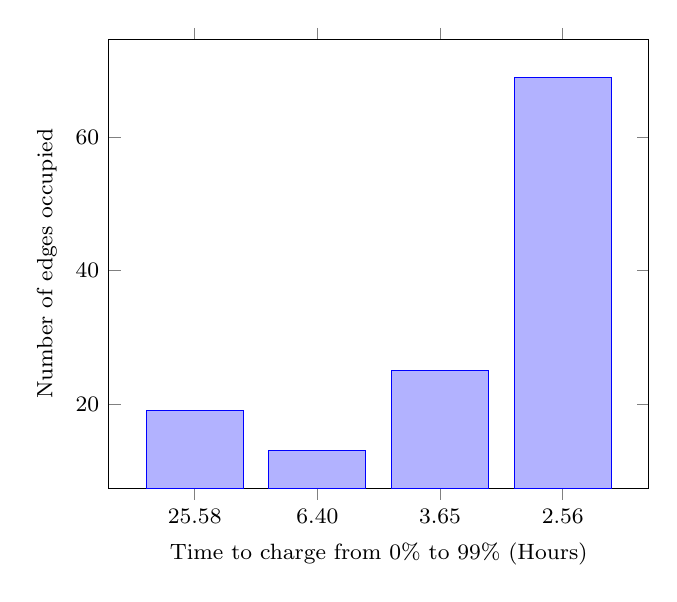
\begin{tikzpicture}
		\begin{axis}[ybar, xmin=0.3, xmax=4.7, font=\footnotesize, xtick={1,2,3,4},xticklabels={25.58, 6.40, 3.65, 2.56},
			ylabel=Number of edges occupied, bar width=35pt, xlabel=Time to charge from 0\% to 99\% (Hours)]
			\addplot coordinates{(1,19) (2,13) (3,25) (4,69)};
		\end{axis}
	\end{tikzpicture}
	\caption{Histogram of charge rates, where each rate is described by how must time it would take to charge a bus from 0\% to 99\%}
	\label{fig:chargeRateHistogram}
\end{figure}













